\documentclass{article}
\usepackage{amsmath}
\usepackage{amssymb}
\usepackage{graphicx}
\usepackage{hyperref}
\usepackage[version=4]{mhchem}


\begin{document}
(2004 AMC 10 A Problem 23) Circles \(A, B\), and \(C\) are externally tangent to each other and internally tangent to circle \(D\).\\
Circles \(B\) and \(C\) are congruent. Circle \(A\) has radius 1 and passes through the center of circle \(D\). What is the radius of circle \(B\) ?\\
(A) \({ }^{\frac{2}{3}}\)\\
(B) \(\frac{\sqrt{3}}{2}\)\\
(C) \(\frac{7}{8}\)\\
(D) \(\frac{8}{9}\)\\
(E) \(\frac{1+\sqrt{3}}{3}\)\\
\centering
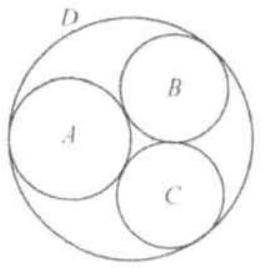
\includegraphics[width=\textwidth]{images/180.jpg}

Solution: (D).\\
Method 1:\\
Let \(E, H\), and \(F\) be the centers of circles \(A, B\), and \(D\), respectively, and let \(G\) be the point of tangency of circles \(B\) and \(C\). Let\\
\(x=F G\) and \(y=G H\).\\
Because circle \(A\) has radius 1 and passes through the center\\
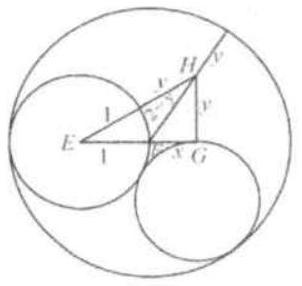
\includegraphics[width=\textwidth]{images/180(2).jpg} of circle \(D\), the radius of circle \(D\) is 2 . Applying the Pythagorean Theorem to right triangles \(E G H\) and \(F G H\) gives \((1+y)^{2}=(1+x)^{2}+y^{2}\), so \(2 y=2 x+x^{2}\),


And \((2-y)^{2}=x^{2}+y^{2}\), so \(4-4 y=x^{2}\).\\
From this it follows that\\
\(x^{2}+\frac{x^{2}}{2}=y=1-\frac{x^{2}}{4}\), so \(0=\frac{3}{4} x^{2}+x-1=\left(\frac{3}{2} x-1\right)\left(\frac{1}{2} x+1\right)\)\\
As a consequence, the two solutions are\\
\(x=\frac{2}{3}, y=1-\frac{(2 / 3)^{2}}{4}=\frac{8}{9}\) and \(x=-2, y=1-\frac{(-2)^{2}}{4}=0\)\\
The radius of circle \(B\) is the positive solution for \(y\), which is \(8 / 9\).

Method 2:\\
We connect the centers of all the circles as shown. \(l\) is the tangent to the circle \(D\). We know that \(G, B\), and \(E\) lie in a straight line.\\
By Heron's formula, \(A=\sqrt{s(s-a)(s-b)(s-c)}\), where \(s=\frac{1}{2}(a+b+c)\)\\
\(=\frac{1}{2}(1+r+1+r+r+r)=2 r+1\).\\
\(A=\sqrt{(2 r+1)(2 r+1-1-r)(2 r+1-r-1)(2 r+1-2 r)}=r \sqrt{2 r+1}\)\\
We also have \(A=\frac{1}{2} B C \times(1+x)=\frac{1}{2} \times(2 r) \times(1+x)=r(1+x)\)\\
So we get \(r(1+x)=r \sqrt{2 r+1}\). Since \(r \neq 0\), we have: \(1+x=\sqrt{2 r+1}\)\\
Applying the Pythagorean Theorem to right triangles \(A B F\) and \(E B F\) gives\\
\((1+r)^{2}-(1+x)^{2}=r^{2}=(2-r)^{2}-x^{2}\)\\
\(\Rightarrow 1+x=3 r-1\)\\
Substituting (1) into (2):\\
\(3 r-1=\sqrt{2 r+1} \quad \Rightarrow \quad(3 r-1)^{2}=2 r+1\)\\
\(\Rightarrow \quad 9 r^{2}-6 r+1=2 r+1 \quad \Rightarrow \quad 9 r^{2}-8 r=0\)\\
\(\Rightarrow \quad r(9 r-8)=0\).\\
\centering

\includegraphics[width=\textwidth]{images/181.jpg}

Since \(r \neq 0\), we have \(r=\frac{8}{9}\).



\end{document}
